% !TEX TS-program = pdflatex
% !TEX encoding = UTF-8 Unicode

% This is a simple template for a LaTeX document using the "article" class.
% See "book", "report", "letter" for other types of document.

\documentclass[11pt]{article} % use larger type; default would be 10pt

\usepackage[utf8]{inputenc} % set input encoding (not needed with XeLaTeX)

%%% Examples of Article customizations
% These packages are optional, depending whether you want the features they provide.
% See the LaTeX Companion or other references for full information.

%%% PAGE DIMENSIONS
\usepackage{geometry} % to change the page dimensions
\geometry{a4paper} % or letterpaper (US) or a5paper or....
% \geometry{margin=2in} % for example, change the margins to 2 inches all round
% \geometry{landscape} % set up the page for landscape
%   read geometry.pdf for detailed page layout information

\usepackage{graphicx} % support the \includegraphics command and options

% \usepackage[parfill]{parskip} % Activate to begin paragraphs with an empty line rather than an indent

%%% PACKAGES
\usepackage{booktabs} % for much better looking tables
\usepackage{array} % for better arrays (eg matrices) in maths
\usepackage{paralist} % very flexible & customisable lists (eg. enumerate/itemize, etc.)
\usepackage{verbatim} % adds environment for commenting out blocks of text & for better verbatim
\usepackage{subfig} % make it possible to include more than one captioned figure/table in a single float
% These packages are all incorporated in the memoir class to one degree or another...
\usepackage[italian]{babel}

%%% HEADERS & FOOTERS
\usepackage{fancyhdr} % This should be set AFTER setting up the page geometry
\pagestyle{fancy} % options: empty , plain , fancy
\renewcommand{\headrulewidth}{0pt} % customise the layout...
\lhead{}\chead{}\rhead{}
\lfoot{}\cfoot{\thepage}\rfoot{}

%%% SECTION TITLE APPEARANCE
\usepackage{sectsty}
\allsectionsfont{\sffamily\mdseries\upshape} % (See the fntguide.pdf for font help)
% (This matches ConTeXt defaults)

%%% ToC (table of contents) APPEARANCE
\usepackage[nottoc,notlof,notlot]{tocbibind} % Put the bibliography in the ToC
\usepackage[titles,subfigure]{tocloft} % Alter the style of the Table of Contents
\renewcommand{\cftsecfont}{\rmfamily\mdseries\upshape}
\renewcommand{\cftsecpagefont}{\rmfamily\mdseries\upshape} % No bold!

%%% END Article customizations

%%% The "real" document content comes below...

\title{Una metodologia di progettazione per hardware riconfigurabile}
\author{Enrico Giordano}
\date{} % Activate to display a given date or no date (if empty),
         % otherwise the current date is printed 

\begin{document}
\maketitle

\section{Introduzione}

Il flusso di progettazione standard di un sistema embedded si divide in tre step: analisi, progettazione e sintesi; questo flusso mira ad avere un sistema specifico per una situazione particolare e alla sintesi finale di tale sistema il meno generale possibile, in modo da renderlo massimamente performante per quel particolare ambiente. 

Con questa tesi, si vuole proporre un approccio alternativo il cui mezzo è l'utilizzo di hardware metamorfico e quindi di una particolare tecnica di progettazione basata sulla ``configurabilità parziale'' della tecnologia delle FPGA. Usando questo mezzo, si vuole progettare un sistema che presenta aspetti embedded (quindi specifici per il target finale) e aspetti più generici e, calato in un contesto particolare, sarà in grado di modificarsi in base alle esigenze ed essere più performante per il contesto in cui viene utilizzato, risparmiando energia, computazioni e memoria. Basandosi sul concetto di ``evoluzione'', secondo cui un oggetto si modifica in base all'ambiente, si otterrà per ogni ambiente un particolare sistema embedded. 

Si presenteranno quindi, a livello descrittivo, le diverse tecniche di configurabilità parziale, introducendo poi un modello di progettazione che mira ad un approccio standardizzato per i futuri sviluppi di questa idea, per poi provare il tutto su un caso di studio reale che possa dimostrare i benefici di questa tecnologia e tecnica di progettazione.

\section{Tecnologia attuale del silicio}
Attualmente esistono 3 tecnologie differenti riguardo l'utilizzo del silicio per scopi computazionali: Hardware General Purpoise, Hardware Embedded e Hardware Riprogrammabile. Queste 3 tipologie differiscono sia per la composizione, sia per la progettazione ma anche per il settore di utilizzo.

\subsection{Hardware General Purpoise}
Questo tipo di Hardware lo si può trovare in processori e microprocessori utilizzati in strumenti di calcolo generici, come PC, moderni telefoni e televisori. La caratteristica peculiare di questi è la generalità: non essendo stati progettati per un sistema specifico, devono permettere di eseguire più operazioni possibili ed essere riprogrammati a piacimento, al limite delle loro potenzialità.

Questi sono composti da un'architettura standard,  rappresentata nella figura  \ref{fig:0}, e viene implementata in ogni CPU, ovvero ciò che implementa questa tecnologia.

\begin{figure}
\centering
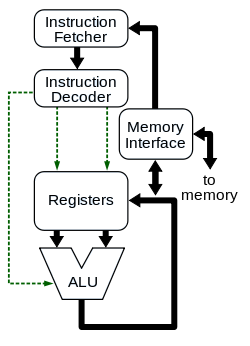
\includegraphics[scale=1]{cpu.png}
\caption{Architettura di una CPU}\label{fig:0}
\end{figure}

Il ciclo di vita di questo hardware è contraddistinto da 3 fasi: fetch, decode, exec; ogni fase è contraddistinta da un insieme di componenti interni utilizzati. La fase di ``fetch'' consiste nel caricare l'istruzione corrente per essere eseguita; la fase di ``decode'' fa in modo che tutti i valori siano disponibili per il calcolo e che l'istruzione possa essere eseguita correttamente impostando i registri interni; la fase di ``exec'' permette, tramite i componenti di memoria e di calcolo (registri e ALU), di eseguire l'istruzione. 

Questo tipo di hardware è molto utile per implementare sistemi generici: la filosofia alla base di questa tecnologia è l'utilizzo più generico possibile, mettendo in secondo piano l'ottimizzazione e il consumo, oltre al costo che cerca di stare relativamente nelle politiche di mercato.

\subsection{Hardware Embedded}
Questo tipo di Hardware è contraddistinto dalla specificità dei suoi componenti interni in base al suo utilizzo; infatti si cerca di utilizzare questo hardware in ambienti o condizioni specifiche, in cui sono richieste operazioni particolari ma soprattutto è necessario ridurre i costi e il consumo dell'applicazione finale.
La tecnologia che rappresenta questo tipo di hardware è una ASIC e difficilmente si trova un'architettura standard, proprio perché l'architettura è specifica per un certo comportamento. Esistono in commercio dei sistemi embedded basati su microprocessori RISC, come ad esempio i Cortex-M della ARM, che hanno un'architettura molto simile a quella delle CPU. In generale comunque ogni ASIC è diversa, in quanto viene mappato su silicio uno specifico algoritmo o un'architettura più complessa.

Un' ASIC deve costare il meno possibile e deve consumare il meno possibile, in base alle esigenze richieste; ovviamente potrà eseguire solo il compito per cui è stata progettata; ha quindi una filosofia di progettazione opposta a quella dell'Hardware General Purpoise.

\subsection{Hardware Riprogrammabile}
L'ultimo tipo di Hardware è quello riprogrammabile, ovvero permette di essere configurato a livello di celle di memoria più volte per implementare diversi comportamenti. Di solito viene utilizzato sia in ambito embedded, per permettere più libertà di progettazione e più efficienza, ma anche a scopo sperimentale, perchè è utile per testare un sistema in fase di sviluppo.

\begin{figure}
\centering
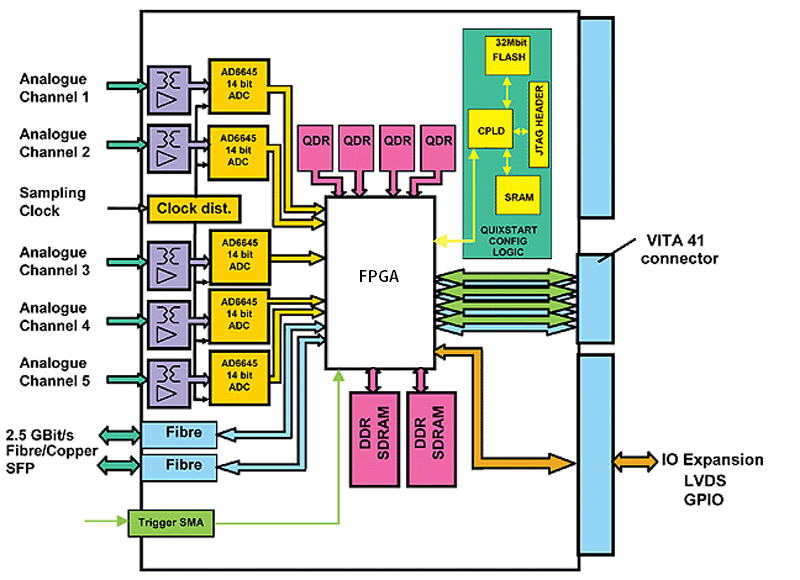
\includegraphics[scale=0.6]{fpga.png}
\caption{Architettura di una FPGA}\label{fig:00}
\end{figure}

Un esempio di architettura (dipende molto dal modello che si vuole utilizzare) lo si può osservare nella figura \ref{fig:00}: la parte riconfigurabile, denotata con FPGA, consiste in un blocco di celle riconfigurabili, che, in base alla descrizione hardware caricata nella memoria flash, possono cambiare struttura. Attorno alla FPGA sono presenti vari moduli standard che possono servire per il consueto utilizzo in ambito di controlli, ma non sempre sono necessarie, in quanto si possono descrivere all'interno della parte riconfigurabile. Parte necessaria per il funzionamento corretto di una FPGA è la logica di controllo della parte riprogrammabile: deve esserci un hardware dedicato per rimappare questa parte, in modo che il processo di riconfigurazione avvenga più velocemente possibile; questo si occuperà quindi di riconfigurare, in base al bitstream che rappresenta l'hardware, la parte riconfigurabile.

In base al suo utilizzo può assumere aspetti di un hardware general purpoise e di un hardware embedded; essendo una tecnologia piuttosto costosa si cerca di utilizzarla il meno possibile, o almeno solo in fase di test.

\section{Il concetto di Hardware Metamorfico}

Il concetto di ``Hardware Metamorfico'' nasce nei primi anni del 1990, per poi perdere parzialmente interesse in quanto veniva presentato come idea, non come tecnologia pratica. Con questo concetto si intende un tipo di Hardware capace di cambiare il proprio comportamento (``evolvere'') utilizzando un ``metodo'' di riconfigurazione: i termini ``evolvere'' e ``metodo'' non sono mai stati definiti in maniera standard, l'articolo che cerca di porre chiarezza su tutto questo ambito \cite{MS1} focalizza l'attenzione sulle diverse sfaccettature del termine ``evoluzione'', parlando di evoluzione ``intrinseca'' , ``estrinseca'' e ``mixata'', rimandando la definizione ad un articolo scientifico precedente \cite{EIE}.

Questo tipo di Hardware è tipico del mondo naturale, in quanto tutti gli oggetti e gli esseri viventi sono in grado di modificarsi in base all'ambiente che li circonda.

\begin{figure}
\centering
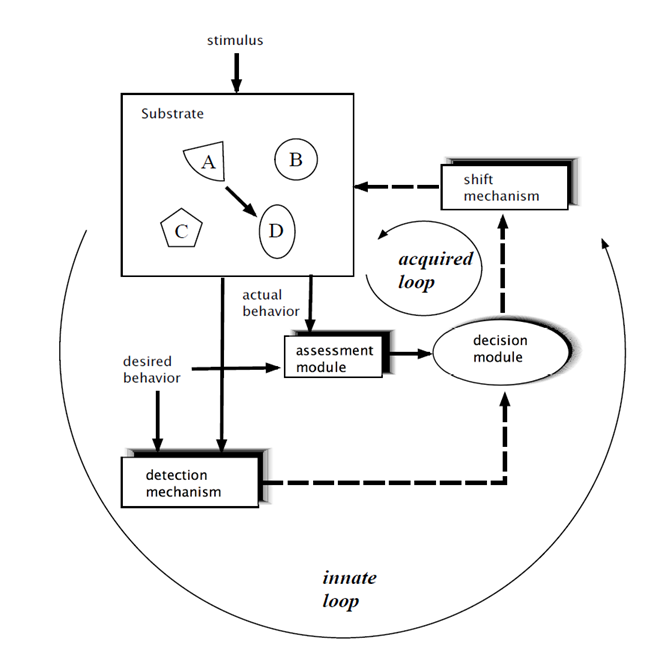
\includegraphics[scale=0.6]{ciclo_evolutivo.png}
\caption{Ciclo evolutivo di un sistema metamorfico}\label{fig:1}
\end{figure}

Il ciclo di vita di un Hardware Metamorfico può essere rappresentato come nella figura \ref{fig:1}: il superciclo che compone questo sistema, chiamato ``ciclo innato'', ha un sotto-ciclo di acquisizione di stimoli, chiamato ``ciclo di acquisizione'', che, tramite il sottostrato di algoritmi di esecuzione, cambia il funzionamento del sistema in base al ``comportamento attuale'' e il ``comportamento desiderato''; con questi dati, tramite un modulo di valutazione degli stimoli e un meccanismo di investigazione (per valutare il comportamento desiderato rispetto al comportamento attuale), viene generato dal modulo di ``decisione'' il risultato che fa modificare l'intero sistema. Il ciclo innato successivamente fa rieseguire questo procedimento, in modo da permettere, potenzialmente all'infinito, la metamorfosi del sistema.

\section{Hardware riconfigurabile}

Per rendere utile l'hardware metamorfico, è necessario trovare una tecnologia che lo rappresenti, in modo da rendere concreto l'utilizzo di tale idea. Per renderla concreta, è necessaria la presenza di un oggetto che possa riprodurre sia il comportamento di silicio, sia il comportamento evolutivo dell'hardware metamorfico. Nel 1985, la Xilinx aveva creato le prime FPGA, rilasciando in commercio il primo modello ``XC2064'', utilizzabile perloppiù per la prototipizzazione di circuiti programmabili. Questa tecnologia sembra prestarsi coerentemente con l'idea di Hardware metamorfico, in quanto è in grado di poter cambiare il proprio comportamento a livello hardware cambiando la propria struttura interna. Il suo carattere riconfigurabile però è stato progettato e utilizzato per la prototipizzazione, non per l'effettivo mutamento di comportamento durante il suo ciclo di vita. 

Nei primi anni `90 nasce una tecnica di progettazione chiamata ``Riconfigurabilità'', da qui poi la tecnologia di applicazione, appunto le FPGA. Questa tecnica consiste nell'utilizzare Hardware con tecnologia riprogrammabile che, tramite la memoria messa a disposizione dentro il sistema, riesce a modificare il suo comportamento. Non è un comportamento appreso completamente dall'ambiente, ma è un comportamento previsto e quindi implementato che va a sostituire un comportamento esistente; il ciclo di vita quindi non sarà composto da un vero e proprio ``apprendimento'', ma sarà una modifica prevista dal progettista. Questo può sembrare limitante, in quanto non c'è piena libertà da parte del dispositivo, ma non avrebbe senso far prendere iniziativa a questo (per i principi della computabilità, non sarebbe nemmeno possibile).

Quindi, più precisamente, si più parlare di ``riconfigurabilità parziale'' e ``riconfigurabilità run-time'': il primo termine pone enfasi su la parziale capacità del dispositivo di modificarsi, in quanto ci sarà una parte progettata che non deve modificarsi ma soprattutto perché il dispositivo non si modificherà completamente, avrà delle modifiche consentite prestabilite; il secondo termine indica il fatto di potersi modificare durante il suo ciclo di vita, cambiando la propria configurazione di porte logiche ottenendo quindi una forma diversa.

\subsection{Metodi di riconfigurazione}

Essendo la Riconfigurabilità una tecnica di progettazione, prevede vari metodi per essere implementata, che possono essere scelti sia per la tecnologia sia in base alle risorse disponibili su essa. Questi metodi sono stati proposti dall'Altera \cite{PR1} e dall'insegnante Dirk Koch , dell'Università di Manchester \cite{PR2}.

La prima tecnica è la ``Riconfigurazione parziale dinamica'', che consiste nel cambiare una parte della FPGA mentre il rimanente circuito continua il suo ciclo di vita. Per fare ciò, esiste una partizione riconfigurabile e in questa si carica il bitstream che corrisponde al nuovo circuito da una memoria esterna. Per far comunicare la parte statica con quella dinamica, è posto un bridge fisico tra di esse. 

Il bridge fisico consiste in un bus, solitamente a 32 bit, che permette lo spostamento di file sintetizzati che rappresentano la nuova configurazione hardware. Questi file si trovano o nella memoria esterna o nella memoria interna, quindi vengono caricati runtime in base a condizioni scelte dal progettista. Solitamente il bus è di tecnologia DMA in modo da essere il più veloce possibile e il trasferimento avviene tramite diversi protocolli gestiti a livello hardware (solitamente il protocollo PCAP a 32 bit, ma dipende dall'architettura ed è trasparente al progettista).

Questa tecnica è molto efficace quando si ha a disposizione poca memoria per memorizzare il bitstream che rappresenta l'hardware e può essere utilizzata in quelle architetture che non dispongono di sufficiente memoria per caricare al completo tutto il sistema descritto.


La seconda tecnica è la ``Rilocazione parziale di bitstream'', che consiste nello ``spostare'' i moduli compilati che descrivono l'hardware (che rappresentano la parte riconfigurabile) da un'area della FPGA all'altra con le stesse dimensioni e proprietà. Questa tecnica è più limitante della precendente, un quanto si pone il vincolo di avere due moduli con stesse dimensioni e proprietà, però può essere utile per questioni di ottimizzazione di codice, in quanto i due moduli possono rappresentare la stessa unità ma al loro interno eseguono lo stesso algoritmo in maniera differente.

\subsection{Readback}

Dal modello ``Virtex 6'' delle FPGA Xilinx, è possibile leggere il contenuto della FPGA e quindi ottenere la configurazione attuale del sistema. Esistono due tipi di lettura: la ``readback verify'', che consiste nella lettura di tutte le celle di memoria, e la ``readback capture'', che permette di leggere le celle di memoria e lo stato dei registri, eseguendo un effettivo dump totale. Questa informazione è di particolare interesse per questo progetto, in quanto permette di ottenere la configurazione ottenuta dopo la metamorfosi, quindi ottenere un nuovo codice. Questa proprietà è stata in parte resa negativa dal punto di vista della sicurezza informatica, in quanto permette di estrapolare codice per poi potenzialmente farne un cattivo uso, però è molto utile per sapere l'andamento della metamorfosi.

\subsection{Metodi di reallocazione}

La parte cruciale quindi di queste tecniche è proprio la reallocazione dei moduli, in quanto la riconfigurabilità consiste proprio nello ``spostare'' un modulo da una sezione attiva a una non attiva. Esistono due modalità di reallocazione: usando dei tools offerti dalla Xilinx e usando il bus.

I tools della Xilinx sono dei software che fungono da middleware per gestire lo spostamento da un'area all'altra e vengono dati in dotazione in base al sistema acquistato. Le direttive del bus sono delle macro da utilizzare durante l'esecuzione del codice per istruire il bus prima di far comunicare i diversi moduli e collegarli. Entrambe le modalità creano un ``ponte'' tra la zona statica e la zona dinamica della logica programmabile, in modo da interconnetterle per generare una nuova descrizione hardware.

Entrambi i metodi si basano sulla riconfigurazione runtime della parte di logica programmabile tramite lo stesso hardware della FPGA che si occupa della riconfigurazione statica (quindi durante la progettazione da parte del progettista), ma in maniera automatica: il modulo di controllo di riconfigurazione sceglie quale può essere la zona di logica programmabile corretta (la prima che ha abbastanza spazio per contenere la nuova logica) e genera il segnale di riconfigurazione; al momento del segnale, si esegue la procedura di riconfigurazione come da prassi ma il bitstream da caricare non deriva da un programma esterno via JTAG bensì dalla memoria interna. Quindi ciò che viene caricato non viene generato runtime, è già presente all'interno della memoria, ma il comportamento globale del sistema cambia in quanto viene caricata una porzione di bitstream che andrà ad alterare il circuito generato dal bitstream statico (che non cambia mai) e quello dinamico (caricato runtime).

\subsection{Aree di reallocazione}

\begin{figure}
\centering
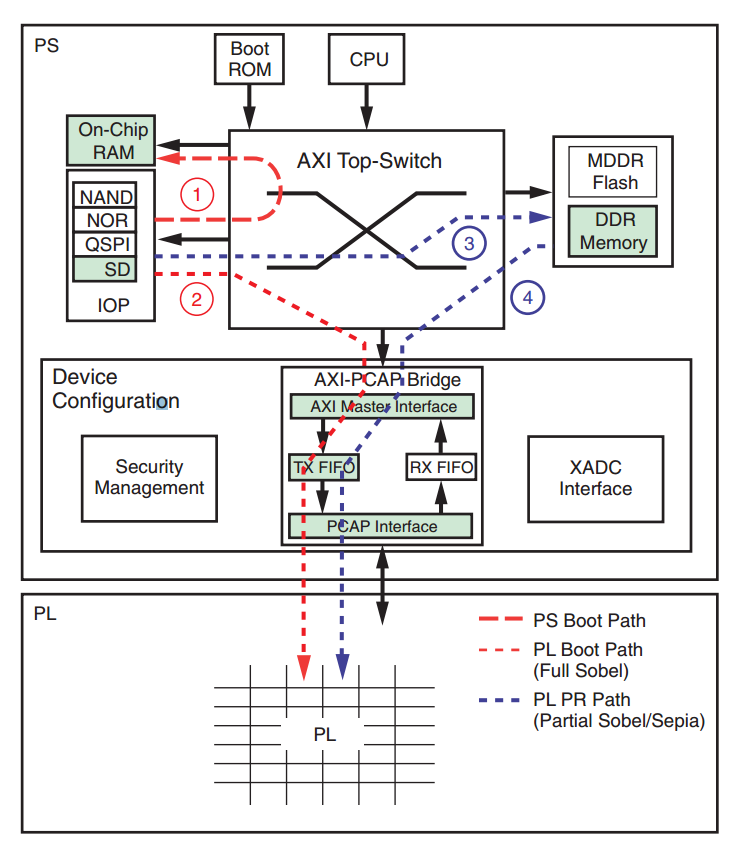
\includegraphics[scale=0.5]{protocollo_riconfigurazione.png}
\caption{Flusso di riconfigurazione}\label{fig:2}
\end{figure}

Il processo di reallocazione visto finora è riassumibile con la figura \ref{fig:2}, in cui si può vedere come la parte di  ``processing system'' (PS) configuri l'informazione da inviare alla parte di ``programmable logic'' (PL) tramite il bridge; caricato il file che rappresenta la nuova parte sintetizzata di programma dalla memoria, si invia alla parte da configurare PL utilizzando il protocollo del bridge.
Le aree precedentemente descritte quindi si trovano all'interno di PL, dove risiede l'effettiva parte logica. Queste aree normalmente possiedono una frammentazione interna ed esterna, in quando il codice non sempre occupa tutti i settori; proprio per questo si può deframmentare e ottenere dei settori vuoti in cui inserire runtime il codice. 

Spostare un nuovo settore dentro la parte di logica programmata significa quindi configurare hardware precedentemente inattivo, dando quindi una nuova configurazione hardware e quindi un diverso comportamento del sistema. In base alla grandezza delle aree da spostare, possono coesistere all'interno dell'area PL, ma non avrebbe senso perché potrebbe significare avere hardware non utilizzato e configurato, quindi si spreca silicio.

\section{La progettazione}

Poichè non esiste un metodo standard per progettare, sviluppare o semplicemente simulare questi sistemi, si vuole creare un nuovo flusso di progettazione per gestire al meglio la fase di sviluppo. Poiché questi sistemi fanno parte di un sottoinsieme dei Sistemi Embedded generici, si utilizzerà ciò che è noto durante la fase di sviluppo di un normale Sistema Embedded per poi aggiungere ciò che serve per specializzare tale sistema in uno Metamorfico.

Il punto di partenza della progettazione non dovrà essere l'analisi dell'ambiente in cui calare il sistema da progettare, bensì sarà scindere cosa deve essere statico e cosa deve essere dinamico: una business logic, ad esempio, può essere una parte statica, mentre un insieme di range su cui fare misure può essere una parte dinamica perché dipende dall'ambiente. Una volta scelte le due parti, si procede con la progettazione come da prassi di un sistema embedded, progettando contemporaneamente queste parti: in questo modo, durante la progettazione, si può capire se le scelte adottate sono state corrette. Infine si configura l'hardware in modo da prepararlo per la sua futura metamorfosi, impostando la parte riconfigurabile, per poi osservare come cambia durante l'acquisizione delle informazioni.

Lo scopo di questa tesi sarà comunque capire come sviluppare al meglio la progettazione di questo tipo di sistema, comprendendo il grado di libertà che si può raggiungere per la parte dinamica e capire quale tipo di riconfigurabilità è più conveniente usare, oltre al fatto di essere sicuri che sia conveniente sfruttare la metamorfosi per risparmiare tempo e denaro durante la progettazione di un sistema embedded.

\section{Simulazione e sintesi di sistemi embedded}

Esistono vari metodi per progettare un sistema embedded; l'approccio ingegneristico più avanzato vuole che si progetti in maniera astratta il sistema, per poi calarlo in un contesto di descrizione tramite HDL per poi eseguire la sintesi. 

\subsection{Simulazione}

Per la descrizione ad alto livello e simulazione, solitamente si utilizza SystemC a diversi livelli, passando da una descrizione mirata a osservare il comportamento dei diversi moduli durante la loro interazione (TLM), fino alla descrizione a livello di EFSM cycle accurate o analogica (RTL e AMS). I vantaggi dell'utilizzo di SystemC sono molteplici, soprattutto grazie allo scheduler interno si riesce a simulare correttamente i vari comportamenti a livello di segnali e attivazione dei moduli.

\subsection{Scheduler di SystemC}

Lo scheduler di SystemC è stato progettato in modo da rispettare una gerarchia di wakeup dei moduli, in quanto l'hardware solitamente è pilotato sia da un clock interno sia da segnali provenienti da diversi moduli, quindi è stato necessario modellare questo parallelismo tramite uno scheduler. Lo schedule eseguito dallo scheduler è diviso in passi:

\begin{enumerate}
\item Elaborazione: vengono create le strutture dati e viene fatto il binding delle porte; 
\item Inizializzazione: vengono inizializzate porte e segnali e vengono fatti eseguire tutti i processi fino alla loro terminazione o al primo wait, in modo da creare una coda d'esecuzione iniziale; 
\item Evaluation: viene fatto eseguire il primo processo pronto in coda d'esecuzione fino alla sua terminazione o ad un wait. Se vengono notificati eventi (con delle notify()), i processi interessati vengono messi in coda d'esecuzione. Se ci sono altri processi in coda pronti ad essere eseguiti ripeto le operazioni precedenti, altrimenti proseguo;
\item Update: vengono aggiornate porte e segnali ed aggiunti in coda d'esecuzione i processi sensibili ad essi; 
\item Delta: vengono aggiunti alla coda d'esecuzione tutti i processi sensibili ad eventuali delta notification (notify(SC\_ZERO\_TIME)) Se ci sono altri processi in coda pronti ad essere eseguiti ripeto le operazioni precedenti a partire dalla fase di evaluation, altrimenti proseguo;
\item Timed: Vengono aggiunti alla coda d'esecuzione tutti i processi sensibili alla prima timed notification (notify(SC\_TIME(n,SC\_NS))). Aggiorno il tempo di simulazione (clock). Se ci sono altri processi in coda pronti ad essere eseguiti ripeto le operazioni precedenti a partire dalla fase di evaluation, altrimenti termino la simulazione. 
\end{enumerate}

Grazie a questo scheduler, si ha uno strumento che simula correttamente un sistema embedded, rispettando anche i tempi accuratamente di esecuzione, osservabili tramite timestamp.

\subsection{Sintesi}

Una volta preparato il modello del sistema in SystemC e simulato correttamente, si procede con la descrizione hardware in HDL, simulazione ed infine sintesi. Solitamente si utilizza VHDL e Verilog, due linguaggi di descrizione hardware che permettono sia di simulare sia di sintetizzare. Solitamente se viene descritto correttamente il sistema in SystemC, il passaggio ad una descrizione HDL è quasi automatico, in quanto si rappresentano gli stessi concetti semanticamente; infatti questo processo dovrebbe essere una traduzione sintattica tra linguaggi.

\section{Simulazione e sintesi di sistemi metamorfici}

Poichè non esiste un metodo standard per progettare sistemi metamorfici, bisogna definire \textit{ex novo} un metodo efficace. Intuitivamente sarebbe consigliato utilizzare la stessa metodologia di progettazione di sistemi embedded standard, in modo da rendere facile l'apprendimento a chi è già abituato a progettare sistemi embedded consuetudinari, oltre a sfruttare le potenzialità di un metodo già assodato e verificato nel tempo.

\subsection{Simulazione con SystemC ReChannel}

Per la simulazione si vorrebbe utilizzare SystemC, in quanto offre una descrizione fedele dell'hardware da simulare e sfrutta la conoscenza di C++ per descrivere i sistemi. Attualmente esiste una libreria di SystemC per la descrizione di sistemi riconfigurabili chiamata ReChannel.

ReChannel è una libreria sviluppata dall'Università di Bonn dal Prof. Armin Felke nel 2008, ceduta a GreenSocs con licenza open-source l'anno successivo e attualmente non più mantenuta, a seguito degli aggiornamenti di SystemC 2.0 che non permettevano la compilazione. La libreria è stata aggiornata e riscritta durante la stesura di questa tesi ed ora è compilabile ed utilizzabile.

La libreria si basa sul concetto di \textbf{switch}, ovvero l'elemento cardine di un sistema riconfigurabile: deve esserci la possibilità di cambiare un modulo con un altro, possibilmente di stessa dimensione e con la stessa quantità di input e output. Lo switch, in questa libreria, viene rappresentato come una sorta di multiplexer, che tiene collegati i diversi moduli della parte riconfigurabile con il modulo della parte statica; al momento opportuno, deciso dal progettista, sia dinamicamente sia staticamente in fase di compilazione, si imposta in modo che attivi il canale di comunicazione tra il modulo attivato e la parte statica, mentre disattiva i moduli della parte dinamica che vengono sostituiti. Lo switch permette la comunicazione sia da parte statica a parte dinamica sia viceversa: la prima viene chiamata \textit{portal}, la seconda viene chiamata \textit{exportal}.

\begin{figure}[ht]
\centering
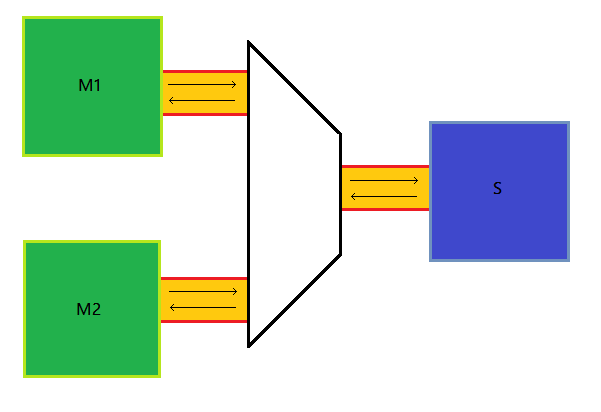
\includegraphics[scale=0.5]{portal.png}
\caption{Rappresentazione dello switch}\label{fig:3}
\end{figure}

Lo switch permette quindi la comunicazione tra i moduli della parte statica e della parte dinamica; la comunicazione può essere semplice (a un solo valore) o multivalore (coda fifo). Questo modella correttamente il concetto di bridge descritto precedentemente, ossia quel componente che permette la comunicazione tra le parti della FPGA. Questo si può vedere come una sorta di bus, che dirige il traffico point to point tra i diversi moduli.

L'utilizzo di questo componente per la comunicazione è un aspetto che si distanzia molto dalla solita progettazione di hardware in SystemC, poiché solitamente si definiscono i moduli con vari input e output e si effettua un collegamento punto-punto all'interno del main; con questa libreria invece si definiscono le modalità di comunicazione tra i moduli di diversa natura, per poi far gestire a questo componente i diversi collegamenti. Questo fatto modella correttamente le FPGA riconfigurabili moderne.

Il problema principale ora, conoscendo lo scheduler di SystemC, è gestire le modalità di schedule dei moduli della parte riconfigurabile; è necessario quindi estendere lo scheduler nativo con delle nuove opzioni.

\begin{figure}[ht]
\centering
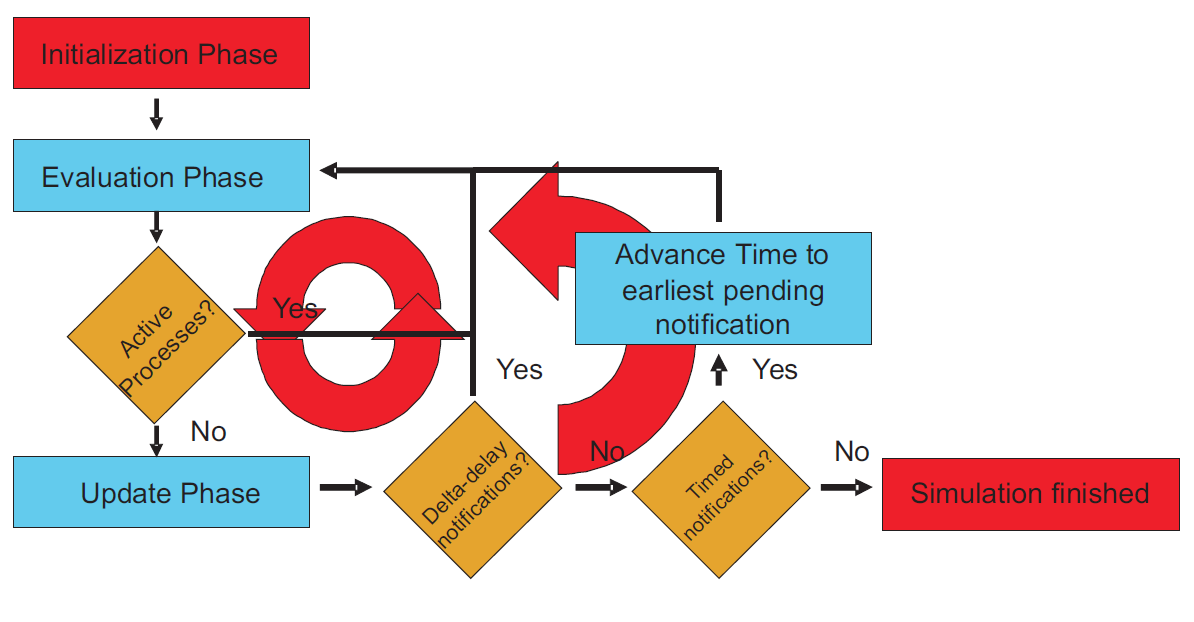
\includegraphics[scale=0.5]{scheduler_rechannel.png}
\caption{Scheduler esteso con ReChannel}\label{fig:4}
\end{figure}

Come si può notare con la figura \ref{fig:4}, è stato esteso lo scheduler dando priorità alla riconfigurazione, quindi nella fase di Evaluation si aggiunge un'ulteriore fase, ovvero il controllo sui processi attivi, oltre ad aggiungere passaggi nella fase di inizializzazione.
Durante la fase di inizializzazione, vengono istanziati tutti i moduli riconfigurabili e disattivati; è compito del progettista decidere quale modulo inizialmente deve essere attivato, ma non è necessario che ci siano moduli attivi. Successivamente, un modulo può essere attivato in qualunque momento; lo scheduler lo attiverà appena entrerà nella parte finale della fase di Evaluation, controllando che ci siano processi attivi pendenti (quindi da attivare).

Solitamente si utilizza un modulo statico che si occupa di fare da transattore tra la parte statica e la parte dinamica; solitamente viene chiamato processo ``Top'' e si occupa sia di descrivere lo switch sia di effettuare la commutazione dei moduli della parte dinamica. Anche in questo caso, viene modellata correttamente l'architettura riconfigurabile, in quando deve esserci un'entità del sistema che si occupa di effettuare la riconfigurazione, che può essere il processore nella board della FPGA o lo stesso progettista se si descrive una riconfigurazione statica.

Un ultimo aspetto molto importante che simula correttamente la realtà è la possibilità di impostare il tempo necessario per la riconfigurazione: ogni modulo, in base alla FPGA target, può metterci tempi differenti per essere attivato e disattivare gli altri, quindi è neccesario un meccanismo per modellare il tempo di riconfigurazione. Questa libreria modella il tempo di riconfigurazione in base al caso pessimo di tempistiche, ovvero permette al progettista di impostare il tempo massimo che impiega il modulo ad essere attivato (infatti non sempre impiega lo stesso tempo per essere riconfigurato, per questo bisogna ragionare per caso pessimo). Può essere deciso questo tempo secondo le specifiche della FPGA target proporzionali all'area che il circuito ricopre (si possono effettuare delle stime in base a quante e quali operazioni vengono eseguite).


\subsection{Sintesi}

La sintesi di questi sistemi è molto simile alla sintesi dei normali sistemi embedded, poiché si utilizza HDL compilato e sintetizzato tramite tool automatici. 

La traduzione da SystemC Rechannel a VHDL è molto semplice: si rappresentano i diversi moduli come moduli statici, contrassegnando i moduli dinamici con un nome riconoscibile ed incrementale (es: reconfigurable\_module1, reconfigurable\_module2, ecc...), ci si assicura che tutto sia stato scritto correttamente e si importano i file nel programma di sintesi prescelto.

Solitamente i programmi di sintesi vengono offerti direttamente dai produttori della FPGA target (ad esempio per la Virtex 4 danno in dotazione il programma) e permettono di impostare facilmente i diversi moduli scritti in HDL tramite interfaccia grafica. Tutti i tool automatici partono quindi dalla descrizione in HDL e, tramite un'ulteriore sforzo del progettista nell'impostare il comportamento dei moduli, acquisiscono la particolarità di essere statici o dinamici.

\begin{figure}[ht]
\centering
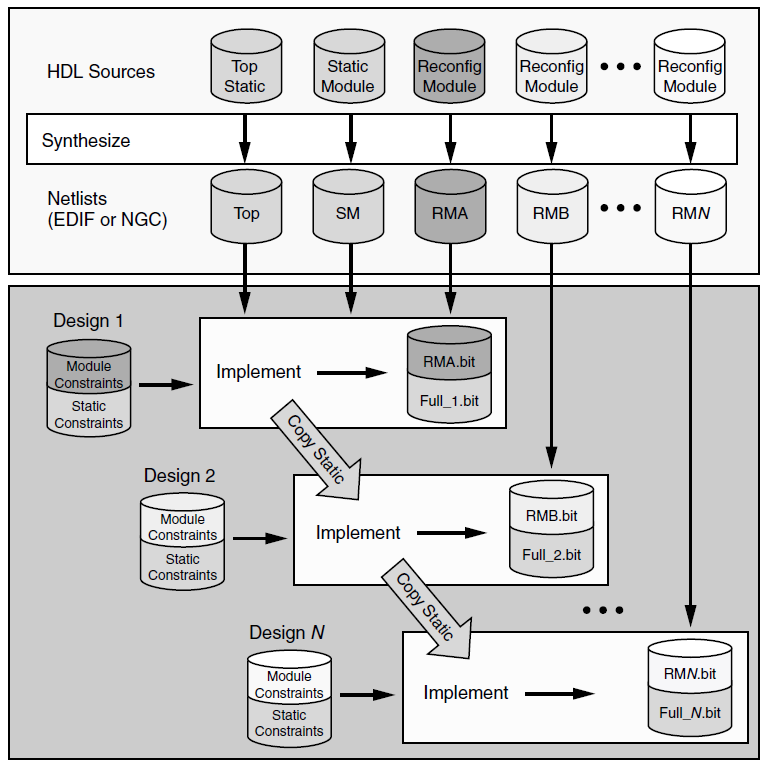
\includegraphics[scale=0.6]{processo_sintesi.png}
\caption{Processo di sintesi eseguito da un tool automatico}\label{fig:5}
\end{figure}

Come si può notare con la figura \ref{fig:5}, il tool automatico identifica i sorgenti come moduli che devono essere sintetizzati; possiamo notare i diversi insiemi di moduli tra cui il modulo ``Top'', già visto precedentemente con SystemC ReChannel, che identifica il transattore tra la parte statica e la parte dinamica del sistema. Una volta sintetizzati i sorgenti, si crea una Netlist, ovvero si creano i collegamenti interni ed esterni tra moduli, in modo da definire il metodo di comunicazione. Fatto ciò, il tool identifica in automatico tutti i differenti design che si creeranno durante il ciclo di vita del sistema, in base alle configurazioni possibili definite nella Netlist; ogni Design è una copia statica presente in memoria, quindi una volta sintetizzata esistono le configurazioni in memoria già pronte per essere nuovamente sintetizzate in hardware (solitamente risiedono nella memoria Flash). 

L'ultimo passaggio del tool automatico è la creazione delle partizioni della FPGA, perché deve essere possibile identificare dove caricare la parte riconfigurabile e dove deve rimanere staticamente il codice; viene creato quindi il file delle partizioni, solitamente chiamato \textit{XPARTITION.xml}, che risiede in memoria e viene consultato ogni volta che deve avvenire una riconfigurazione.


\begin{thebibliography}{1}
\bibitem{MS1} Garrison W. Greenwood,Senior Member, IEEE and Andy M. Tyrrell,Senior Member, IEEE, ``\textit{Metamorphic Systems: A New Model for Adaptive System Design''}, 2010
\bibitem{EIE} Sekanina, L. ; Brno Univ. of Technol., Brno ; Martinek, T. ; Gajda, Z., \textit{Extrinsic and Intrinsic Evolution of Multifunctional Combinational Modules}, 2006
\bibitem{PR1} Altera, \textit{FPGA Run-Time Reconfiguration: Two Approaches}, 2008
\bibitem{PR2} Dirk Koch, \textit{Partial Reconfiguration on FPGAs}, 2013
\bibitem{Rechannel} Raabe A., Tech. Comput. Sci., Univ. of Bonn, Felke A., \textit{A SYSTEMC language extension for high-level reconfiguration modelling}, 2008
\bibitem{Rechannel2} Erlangung des Doktorgrades, Mathematisch-Naturwissenschaftlichen Fakultat, Rheinischen Friedrich-Wilhelms-Universitat Bonn, \textit{Describing and Simulating Dynamic Reconfiguration in SystemC Exemplified by a Dedicated 3D Collision Detection Hardware}, 2008
\end{thebibliography}

\end{document}
